% ==============================================================================
% 第三章 直觀機率
% ==============================================================================
\section{直觀機率}\label{sec:b5-ch3}

\begin{center}
\begin{minipage}{0.75\textwidth}
\begin{itemize}[leftmargin=2em, itemsep=0.3em]
  \item[§ III-1] \textbf{機率定義及基本性質}
  \item[§ III-2] \textbf{機率求法}
  \item[*§ III-3] \textbf{幾何機率}
\end{itemize}
\end{minipage}
\end{center}

\begin{center}
$* \qquad * \qquad * \qquad * \qquad *$
\end{center}

對於若干應用問題，我們可以根據已知條件，列出方程式，而求得確定的答案．但是也有很多問題，本身包含偶然的因素，而沒有必然的確定結果．對於這一類問題，我們就必須根據這些偶然的因素來作推斷．例如氣象預報、骰子遊戲等，我們知道那些結果會出現，但是並不能肯定其中某一個結果必然出現．機率理論就是討論各種偶然事件的數學理論，尋求偶然事件所遵循的規則．

機率理論的起源也很偶然，在 1654 年一位賭徒向巴斯卡 (Blaise Pascal) 請教一項賭注的分配問題．巴斯卡與另一位法國數學家費瑪 (Pierre Fermat) 用排列組合方法共同討論這一個機會遊戲問題．他們兩人的討論就是有系統研究機率理論的開始，以後機率理論逐漸發展，應用的範圍也日益擴大．今天，機率理論已成為現代科學中一個重要部份，應用範圍包含自然科學以及生物、醫學、農業、工業、政治、經濟等各方面．另一方面，機率理論對於統計學的發展也有非常重大的貢獻．

下面是機率理論發展史上的幾個重要而有趣的例子，給大家參考．

\medskip
\noindent\textbf{【骰子問題】}義大利的托斯卡尼大公爵，喜作骰子戲，每次擲三顆骰子時，出現10點的次數比 9 點多，但是10與 9 都各有 6 種分割方法：
\begin{align*}
10 &= 6 + 3 + 1 = 6 + 2 + 2 = 5 + 4 + 1 = 5 + 3 + 2 \\
   &= 4 + 4 + 2 = 4 + 3 + 3, \\
9  &= 6 + 2 + 1 = 5 + 3 + 1 = 5 + 2 + 2 = 4 + 4 + 1 \\
   &= 4 + 3 + 2 = 3 + 3 + 3.
\end{align*}
二者出現的頻繁程度似乎應該相同才對．據說他向加利略 (Galileo Galilei 1564--1642) 提出這個問題，由加利略給予解答．加利略求出出現10點的情形有27種，而出現 9 點的情形只有25種．(請讀者自行驗證)

加利略的這個結果是有關機率的一項最早的紀錄，現在我們不難用前一章的排列方法算出這個結果．

\medskip
\noindent\textbf{【賭注分配問題】}甲、乙二人作對局遊戲，二人獲勝的機會均等，誰先勝三局可得一筆賭注，進行至甲勝兩局，乙勝一局時，發生緊急事故遊戲必需中止．因此應該依照一種公平原則將賭注分給甲、乙二人，巴斯卡與費瑪依照各人先勝三局的機會，主張甲應分得賭注的 3/4，乙應分得 1/4．

這個例子就是上面所說的研究機率理論的起點．

\medskip
\noindent\textbf{【全盤獲勝問題】}甲有 $m$ 元，乙有 $n$ 元，二人作擲一枚公正的（卽正反面出現的機會均等）硬幣遊戲，出現正面則甲贏乙一元，出現反面則乙贏甲一元，問甲將乙所有的全部資本 $n$ 元贏去的機會爲多少？這個問題顯然與甲、乙二人所有的資本有關，答案爲
\[
\frac{m}{m+n}.
\]
這個問題的答案看上去很簡單，但是導出這個答案的過程卻有點複雜．(解法請參閱 §III-2，論例 8)

上面這些早期的有關機會遊戲的例子，到現在仍然是機率理論中的典型例題．這是因爲關於投硬幣與擲骰子的討論具有相當的代表性，很容易引伸到一般情形．因此在以下的討論中，我們也常利用硬幣和骰子來舉例說明．

% ==============================================================================
% § III-1 機率定義及基本性質
% ==============================================================================
\subsection{機率定義及基本性質}\label{sec:b5-3-1}

概略地說，機率就是用來衡量一項事件可能出現的程度．我們用 0 與 1 之間的實數表示機率的大小；機率爲 0 時表示這項事件絕不可能發生，而機率爲 1 時則表示這項事件必然發生．一項事件的機率有時由直觀認定，例如投硬幣時出現正面的機率爲 $\frac{1}{2}$；有時則由經驗而賦予，例如產品的損壞率，棒球選手的打擊率等．

\medskip
\noindent\textbf{定義}\quad 一項試驗中所有可能發生的現象形成的集合稱爲\textbf{樣本空間} (Sample space 也叫做基集)，用 $S$ 表示，$S$ 中每一點(卽每一可能發生的現象)稱爲一個\textbf{樣本點} (Sample point) 或\textbf{基本事件} (elementary event)．

在本書中沒有特別說明時，只考慮 $S$ 爲有限的情形．

\medskip
\noindent\textbf{定義}\quad 設樣本空間 $S$ 爲有限，$S$ 的每一子集 $A$ 稱爲\textbf{一項事件}．空集合 $\phi$ 稱爲\textbf{空事件}，$S$ 本身稱爲\textbf{全事件}．$A$ 在 $S$ 中的補集 $A'=S-A$ 稱爲 $A$ 的\textbf{餘事件}．若 $B$ 爲 $S$ 的另一子集，則聯集 $A \cup B$ 稱爲 $A$ 與 $B$ 的\textbf{和事件}，而交集 $A \cap B$ 稱爲 $A$ 與 $B$ 的\textbf{積事件}．

若 $A \cap B = \phi$，我們則說 $A, B$ 二事件\textbf{互斥}．

我們把各名詞用下表列出，看起來比較清楚：

\begin{center}
\renewcommand{\arraystretch}{1.2}
\begin{tabular}{l|l}
\hline
$S$ & 樣本空間 \\
$a\,(\in S)$ & 樣本點或基本事件 \\
$A\,(\subset S)$ & 事件 \\
$\phi$ & 空事件 \\
$S$ & 全事件 \\
$A'=S-A$ & 餘事件 \\
$A, B \subset S,\quad A \cup B$ & 和事件 \\
$A \cap B$ & 積事件 \\
$A, B\,(A \cap B = \phi)$ & 二事件互斥 \\
\hline
\end{tabular}
\end{center}

下面是簡單的圖示，可以幫助了解：

\begin{figure}[H]
\centering
\begin{tikzpicture}[scale=0.95]
  % (a) a \in S
  \begin{scope}[shift={(0,0)}]
    \draw[thick] (0,0) circle (1.1);
    \node at (50:1.35) {$S$};
    \fill (-0.2,-0.1) circle (2pt) node[right=2pt] {$a$};
    \node at (0,-1.55) {$a \in S$};
  \end{scope}

  % (b) A 與 A'
  \begin{scope}[shift={(2.9,0)}]
    \draw[thick] (0,0) circle (1.1);
    \node at (50:1.35) {$S$};
    \draw[thick] (115:1.1) to[out=-60, in=60] (245:1.1);
    \node at (-0.45, 0.05) {$A$};
    \node at (0.45, 0.05) {$A'$};
    \node at (0,-1.55) {$A \text{ 與 } A'$};
  \end{scope}

  % (c) A \cup B
  \begin{scope}[shift={(5.8,0)}]
    \draw[thick] (0,0) circle (1.1);
    \node at (50:1.35) {$S$};
    
    % Hatch union of A and B
    \begin{scope}
      \clip (0,0) circle (1.1);
      \fill[pattern=north east lines, pattern color=black!70] 
        (-0.25, 0.15) circle (0.6)
        (0.25, -0.2) circle (0.6);
    \end{scope}
    
    \draw[thick] (-0.25, 0.15) circle (0.6);
    \draw[thick] (0.25, -0.2) circle (0.6);
    
    \node at (-0.45, 0.25) {$A$};
    \node at (0.45, -0.3) {$B$};
    \node at (0,-1.55) {$A \cup B$};
  \end{scope}

  % (d) A \cap B
  \begin{scope}[shift={(8.7,0)}]
    \draw[thick] (0,0) circle (1.1);
    \node at (50:1.35) {$S$};
    
    % Hatch intersection of A and B
    \begin{scope}
      \clip (-0.25, 0.15) circle (0.6);
      \fill[pattern=north east lines, pattern color=black!70] (0.25, -0.2) circle (0.6);
    \end{scope}
    
    \draw[thick] (-0.25, 0.15) circle (0.6);
    \draw[thick] (0.25, -0.2) circle (0.6);
    
    \node at (-0.5, 0.25) {$A$};
    \node at (0.5, -0.3) {$B$};
    \node at (0,-1.55) {$A \cap B$};
  \end{scope}
\end{tikzpicture}
\caption*{圖 3-1}
\label{fig:b5-3-1}
\end{figure}

\noindent
\begin{minipage}[c]{0.58\textwidth}
\textbf{【論例 1】}擲一粒骰子一次，則樣本空間可寫爲
\[
S=\{1, 2, 3, 4, 5, 6\}.
\]
\end{minipage}\hfill
\begin{minipage}[c]{0.38\textwidth}
\centering
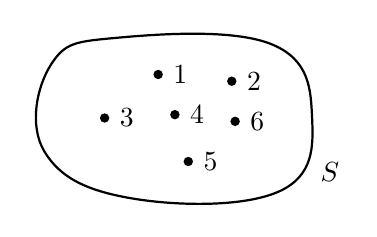
\begin{tikzpicture}[scale=0.85]
  \draw[thick] plot[smooth cycle, tension=0.7] coordinates {
    (0, 1.2) (2.3, 1.1) (2.9, 0) (2.4, -1.1) (0.2, -1.2) (-1.1, -0.5) (-1.0, 0.8)
  };
  \node[right=2pt] at (2.8, -0.8) {$S$};
  
  \fill (0.6, 0.65) circle (2pt) node[right=2pt] {$1$};
  \fill (1.7, 0.55) circle (2pt) node[right=2pt] {$2$};
  \fill (-0.2, 0.0) circle (2pt) node[right=2pt] {$3$};
  \fill (0.85, 0.05) circle (2pt) node[right=2pt] {$4$};
  \fill (1.75, -0.05) circle (2pt) node[right=2pt] {$6$};
  \fill (1.05, -0.65) circle (2pt) node[right=2pt] {$5$};
\end{tikzpicture}
\par\vspace{0.2em}
{\small 圖 3-2}
\end{minipage}

\medskip
可能出現的點數就是一個基本事件，設 $A$ 表示出現偶數的事件，則 $A=\{2, 4, 6\}$，$A$ 的餘事件 $A'=S-A=\{1, 3, 5\}$，卽表示出現奇數的事件，$A$ 與 $A'$ 的和事件 $A \cup A' = S$ 就是全事件．因 $A \cap A' = \phi$，故 $A$ 與 $A'$ 互斥，卽表示偶數與奇數不可能同時出現．

在本章中我們只考慮樣本空間中各基本事件有均等機會出現的情形（雖然實際情形並不一定如此，但與這種理想的情況極爲接近），可定義機率如下：

\medskip
\noindent\textbf{定義}\quad 設樣本空間 $S$ 爲有限，$|S|=n$，且其中各基本事件出現的機率均等．若 $A \subset S$ 爲一事件，$|A|=k$，則定義事件 $A$ 的機率爲 $\frac{k}{n}$，記作
\[
P(A) = \frac{k}{n}.
\]
這個定義最初由拉普拉士 (Laplace 1749--1827) 所給予，所以就叫做拉普拉士的古典定義．

\medskip
\noindent\textbf{〔例 1〕} 擲骰子一粒，出現偶數點的機率是多少？

\indent\textbf{解}\quad 樣本空間 $S=\{1, 2, 3, 4, 5, 6\}$，$|S|=6$．出現偶數點的事件 $A=\{2, 4, 6\}$，$|A|=3$．故所求機率 $P(A) = 3/6 = 1/2$．\hfill $\#$

\medskip
\noindent\textbf{〔例 2〕} 某期愛國獎券發行 60 萬張，某君購買 100 張，問中第一特獎的機率是多少？

\indent\textbf{解}\quad 在此情形 $|S|=600000$，$|A|=100$，故
\[
P(A) = \frac{100}{600000} = \frac{1}{6000}.
\]

\medskip
\noindent\textbf{〔例 3〕} 袋中有紅球 5 個，白球 2 個，大小都相同．問一次取出一紅球的機率是多少？

\indent\textbf{解}\quad $|S|=7$．設取得一紅球的事件爲 $A$，則 $|A|=5$，因此
\[
P(A) = \frac{5}{7}. \tag*{\#}
\]

\medskip
\noindent\textbf{〔例 4〕} 擲硬幣兩次，兩次出現同一面的機率是多少？

\indent\textbf{解}\quad 樣本空間可寫爲 $S=\{(\text{正}, \text{正}), (\text{正}, \text{反}), (\text{反}, \text{正}), (\text{反}, \text{反})\}$．

出現同一面的事件 $A=\{(\text{正}, \text{正}), (\text{反}, \text{反})\}$，故 $P(A) = \frac{2}{4} = \frac{1}{2}$．\hfill $\#$

\medskip
由機率的定義我們可以直接得到下列性質：
\begin{enumerate}[label=\Roman*., itemsep=2pt, topsep=2pt]
  \item 空事件的機率爲 0：$P(\phi) = 0$．
  \item 全事件的機率爲 1：$P(S)=1$．
  \item 一般事件的機率在 0 與 1 之間：$0 \le P(A) \le 1$．
  \item 加法性：若 $A \cap B = \phi$，則 $P(A \cup B) = P(A) + P(B)$．
  \item 和事件的機率：$P(A \cup B) = P(A) + P(B) - P(A \cap B)$．
  \item 餘事件的機率：$P(A') = 1 - P(A)$．
  \item 單調性：若 $A \subset B$，則 $P(A) \le P(B)$．
\end{enumerate}

\medskip
\noindent\textbf{證明}\quad 性質 I--III 顯然成立，我們來證性質 IV：因 $A \cap B = \phi$，故 $|A \cup B| = |A| + |B|$．於是
\begin{align*}
P(A \cup B) &= \frac{|A \cup B|}{|S|} = \frac{|A| + |B|}{|S|} = \frac{|A|}{|S|} + \frac{|B|}{|S|} \\
&= P(A) + P(B).
\end{align*}
性質 V 的證明留作習題，由於 $A \cup A' = S$ 及 $A \cap A' = \phi$，由 IV 得
\[
P(A) + P(A') = P(A \cup A') = 1,
\]
這就是性質 VI．最後證明性質 VII：設 $A \subset B$，則
\[
B = A \cup (B - A) \text{ 且 } A \cap (B - A) = \phi,
\]
故由 IV 及 III 可得
\[
P(B) = P(A) + P(B - A) \ge P(A). \tag*{\#}
\]

\medskip
\noindent\textbf{【論例 2】}擲骰子三次，設三次中至少出現一次 6 點的事件爲 $A$，三次中至少出現一次 1 點的事件爲 $B$，試求 $P(A'), P(A), P(B), P(A \cap B)$ 及 $P(A \cup B)$．

\indent\textbf{解}\quad 設 $T=\{1, 2, 3, 4, 5, 6\}$，則樣本空間 $S=T^3$，$|S|=6^3=216$，$A$ 的餘事件 $A'$ 表示三次中未出現 6 點的事件，故 $|A'|=5^3=125$，因此
\[
P(A') = \frac{125}{216},
\]
\[
P(A) = 1 - P(A') = 1 - \frac{125}{216} = \frac{91}{216}.
\]\phantomsection\label{note:b5-ch3-p99-pa}\footnote{【原書註記/校訂】：原書誤植為「$P(A)=P(A')=1-\frac{125}{216}=\frac{91}{216}$」，第二個等號左側漏印「$1-$」，茲更正為「$P(A)=1-P(A')$」．}
同理，
\[
P(B) = \frac{91}{216}.
\]
用排列方法算出 $|A \cap B| = 30$，得
\[
P(A \cap B) = \frac{30}{216}.
\]
因此，
\begin{align*}
P(A \cup B) &= P(A) + P(B) - P(A \cap B) = \frac{91}{216} + \frac{91}{216} - \frac{30}{216} \\
&= \frac{151}{216}.
\end{align*}

性質 IV（加法性）可以推廣到任意有限多個事件的情形：

\medskip
\noindent\textbf{IV$'$.} 設 $k$ ($k \ge 2$) 個事件 $A_1, A_2, \dots, A_k$ 中任意二事件皆爲互斥，則
\[
P(A_1 \cup A_2 \cup \cdots \cup A_k) = P(A_1) + P(A_2) + \cdots + P(A_k).
\]

\medskip
\noindent\textbf{證明}\quad 利用數學歸納法．$k=2$ 時由 IV 上式成立．假定 $k$ 時成立．$k+1$ 時，因 $A_i \cap A_j = \phi$，$i \ne j$，故 $(A_1 \cup \cdots \cup A_k) \cap A_{k+1} = \phi$，因此
\begin{align*}
P(A_1 \cup \cdots \cup A_{k+1}) &= P[(A_1 \cup \cdots \cup A_k) \cup A_{k+1}] \\
&= P(A_1 \cup \cdots \cup A_k) + P(A_{k+1}) \quad \text{（由 IV）．}
\end{align*}
又由歸納法的假設，得
\[
P(A_1 \cup \cdots \cup A_k) = P(A_1) + \cdots + P(A_k),
\]
代入上式卽得
\[
P(A_1 \cup \cdots \cup A_{k+1}) = P(A_1) + \cdots + P(A_{k+1}). \tag*{\#}
\]

\medskip
\noindent\textbf{定義}\quad 設 $A$ 爲樣本空間 $S$ 中的一個非空事件，$B$ 爲 $S$ 中的一個任意事件，我們定義在 $A$ 出現之下，$B$ 出現的\textbf{條件機率}爲
\[
P(B \mid A) = \frac{P(A \cap B)}{P(A)}
\]
我們不難推得下列結果：

\medskip
\noindent\textbf{VIII.} 乘法性\quad 設 $A$ 爲非空事件，則
\[
P(A \cap B) = P(A) P(B \mid A).
\]

\medskip
\noindent\textbf{VIII$'$.} 設 $A_1, \dots, A_k$ 皆爲非空事件，且 $A_1 \cap \cdots \cap A_k \ne \phi$，則
\begin{align*}
P(A_1 \cap \cdots \cap A_k) &= P(A_1) P(A_2 \mid A_1) P(A_3 \mid A_1 \cap A_2) \\
&\quad \cdots P(A_k \mid A_1 \cap \cdots \cap A_{k-1}).
\end{align*}

\medskip
\noindent\textbf{VIII之證明}\quad 因 $P(A) \ne 0$，故由定義得
\[
P(A \cap B) = P(A) P(B \mid A). \tag*{\#}
\]

\medskip
\noindent\textbf{VIII$'$之證明}\quad 利用數學歸納法證明，當 $k=2$ 時由 VIII 成立．假定 $k$ 時成立，當 $k+1$ 時，由 VIII 得
\begin{align*}
P(A_1 \cap \cdots \cap A_k \cap A_{k+1}) &= P[(A_1 \cap \cdots \cap A_k) \cap A_{k+1}] \\
&= P(A_1 \cap \cdots \cap A_k) P(A_{k+1} \mid A_1 \cap \cdots \cap A_k).
\end{align*}
由歸納法的假設
\[
P(A_1 \cap \cdots \cap A_k) = P(A_1) P(A_2 \mid A_1) \cdots P(A_k \mid A_1 \cap \cdots \cap A_{k-1})
\]
代入上式卽得 VIII$'$．

\medskip
\noindent\textbf{定義}\quad 設 $A, B$ 皆爲非空事件．若
\[
P(A \cap B) = P(A) P(B)
\]
成立，則稱 $B$ 與 $A$ 無關，或稱 $A, B$ 二事件\textbf{互爲獨立}．

由獨立事件的定義，VIII 可化簡爲下列公式：

\medskip
\noindent\textbf{IX.} $A, B$ 二事件互爲獨立 $\Longleftrightarrow P(B \mid A) = P(B)$．

\medskip
\noindent\textbf{定義}\quad 設 $A, B, C$ 是三個非空事件．若其中每一對皆互爲獨立事件，而且
\[
P(A \cap B \cap C) = P(A) P(B) P(C)
\]
成立，則稱 $A, B, C$ 之事件爲\textbf{獨立}．

\medskip
\noindent\textbf{【論例 3】}袋中有三紅球，二白球，每次採取一球不放回，問紅球先取完的機率是多少？

\indent\textbf{解}\quad 紅球先取完的事件爲下列 4 種：
\begin{enumerate}[1.]
  \item 紅紅紅，
  \item 紅紅白紅，
  \item 紅白紅紅，
  \item 白紅紅紅．
\end{enumerate}
顯然此 4 事件爲互斥，其中一種發生時其他不會同時發生，故由 ($\text{IV}'$) 加法性可知所求機率爲此 4 事件的機率的和．各事件機率的求法如下：

先考慮紅紅紅之事件的機率．第一次取出紅球（設爲事件 $A_1$）的機率爲 $\frac{3}{5}$，卽 $P(A_1) = \frac{3}{5}$．第一次出現紅球（事件 $A_1$）之下（卽袋中剩下 2 紅球，2 白球），第二次取出紅球（設爲事件 $A_2$）的條件機率爲 $\frac{2}{4}$，卽 $P(A_2 \mid A_1) = \frac{2}{4}$．第一，二次均出現紅球（卽事件 $A_1 \cap A_2$）之下（袋中剩下 1 紅球，2 白球），第三次取出紅球（設爲事件 $A_3$）的條件機率爲 $\frac{1}{3}$，卽 $P(A_3 \mid A_1 \cap A_2) = \frac{1}{3}$，因此第一，二，三次均出現紅球（卽事件 $A_1 \cap A_2 \cap A_3$）的機率由 ($\text{VIII}'$) 可得
\begin{align*}
P(A_1 \cap A_2 \cap A_3) &= P(A_1) P(A_2 \mid A_1) P(A_3 \mid A_1 \cap A_2) \\
&= \frac{3}{5} \cdot \frac{2}{4} \cdot \frac{1}{3} = \frac{1}{10}.
\end{align*}
同理可得
\begin{align*}
\text{紅紅白紅的機率爲 } &\frac{3}{5} \cdot \frac{2}{4} \cdot \frac{2}{3} \cdot \frac{1}{2} = \frac{1}{10}, \\
\text{紅白紅紅的機率爲 } &\frac{3}{5} \cdot \frac{2}{4} \cdot \frac{2}{3} \cdot \frac{1}{2} = \frac{1}{10}, \\
\text{白紅紅紅的機率爲 } &\frac{2}{5} \cdot \frac{3}{4} \cdot \frac{2}{3} \cdot \frac{1}{2} = \frac{1}{10}.
\end{align*}
因此紅球先取完的機率爲
\[
\frac{1}{10} + \frac{1}{10} + \frac{1}{10} + \frac{1}{10} = \frac{2}{5}.
\]

\medskip
\noindent\textbf{【論例 4】}投一枚公正的銅錢三次，第一次出現正面的事件設爲 $A$，第二次出現正面的事件設爲 $B$，第三次出現反面的事件設爲 $C$．試問 $A, B, C$ 是否獨立？

\indent\textbf{解}\quad 樣本空間
\begin{align*}
S &= \{(\text{正}, \text{正}, \text{正}), (\text{正}, \text{正}, \text{反}), (\text{正}, \text{反}, \text{正}), (\text{反}, \text{正}, \text{正}), \\
  &\phantom{{}=\{ \ \ } (\text{反}, \text{反}, \text{正}), (\text{反}, \text{正}, \text{反}), (\text{正}, \text{反}, \text{反}), (\text{反}, \text{反}, \text{反})\}; \\
A &= \{(\text{正}, \text{正}, \text{正}), (\text{正}, \text{正}, \text{反}), (\text{正}, \text{反}, \text{正}), (\text{正}, \text{反}, \text{反})\}, \\
B &= \{(\text{正}, \text{正}, \text{正}), (\text{正}, \text{正}, \text{反}), (\text{反}, \text{正}, \text{正}), (\text{反}, \text{正}, \text{反})\}, \\
C &= \{(\text{正}, \text{正}, \text{反}), (\text{反}, \text{正}, \text{反}), (\text{正}, \text{反}, \text{反}), (\text{反}, \text{反}, \text{反})\}; \\
A \cap B &= \{(\text{正}, \text{正}, \text{正}), (\text{正}, \text{正}, \text{反})\}, \\
B \cap C &= \{(\text{正}, \text{正}, \text{反}), (\text{反}, \text{正}, \text{反})\}, \\
C \cap A &= \{(\text{正}, \text{正}, \text{反}), (\text{正}, \text{反}, \text{反})\}; \\
A \cap B \cap C &= \{(\text{正}, \text{正}, \text{反})\}.
\end{align*}
\[
P(A) = P(B) = P(C) = \frac{4}{8} = \frac{1}{2},
\]
\[
P(A \cap B) = P(B \cap C) = P(C \cap A) = \frac{2}{8} = \frac{1}{4},
\]
\[
P(A \cap B \cap C) = \frac{1}{8}.
\]
\[
P(A \cap B) = P(A)P(B),\quad P(B \cap C) = P(B)P(C),\quad P(C \cap A) = P(C)P(A).
\]
\[
P(A \cap B \cap C) = P(A)P(B)P(C).
\]
因此 $A, B, C$ 爲獨立事件．

\medskip
\noindent\textbf{【論例 5】}投一枚公正的銅錢三次，其中恰有兩次爲正面的機率如何？

\indent\textbf{解}\quad 三次中恰有兩次正面的事件有下列 $3$ ($=C_2^3$) 種：
\begin{enumerate}[1.]
  \item 正正反，
  \item 正反正，
  \item 反正正．
\end{enumerate}
此三種事件顯然互斥，故所求機率爲此三事件的機率和．

由論例 4 得知第一次出現正面，第二次出現正面，第三次出現反面之三事件獨立，故正正反之事件的機率爲 $\frac{1}{2} \cdot \frac{1}{2} \cdot \frac{1}{2} = \frac{1}{2^3}$．同樣地，正反正，反正正二事件的機率亦各爲 $\frac{1}{2^3}$．因此所求機率爲
\[
\frac{1}{2^3} + \frac{1}{2^3} + \frac{1}{2^3} = C_2^3 \left(\frac{1}{2}\right)^3 = \frac{3}{8}. \tag*{\#}
\]

% ==============================================================================
% 習題 III-1
% ==============================================================================
\subsubsection*{習題 III-1}\label{sec:b5-ex3-1}

\begin{enumerate}[label=\textbf{\arabic*.}]
  \item 
  \begin{enumerate}[label=(\arabic*)]
    \item 設 $A, B$ 爲有限集合 $S$ 的子集，試證
    \[
    |A \cup B| = |A| + |B| - |A \cap B|
    \]
    \item 利用上述關係證明，對於樣本空間 $S$ 中任二事件 $A, B$，下述關係成立：
    \[
    P(A \cup B) = P(A) + P(B) - P(A \cap B)
    \]
  \end{enumerate}

  \item 令 $A, B, C$ 爲樣本空間 $S$ 中的三個事件，利用題 1 (2) 證明
  \[
  P(A \cup B \cup C) = P(A) + P(B) + P(C) - P(A \cap B) - P(B \cap C) - P(C \cap A) + P(A \cap B \cap C).
  \]

  \item 擲五枚硬幣，五枚都不是正面的機率是多少？至少有一枚是正面的機率是多少？

  \item 擲五粒骰子，兩粒出現都不是 6 點的機率是多少？至少有一粒是 6 點的機率是多少？\phantomsection\label{note:b5-ch3-p104-q4}\footnote{【原書註記/校訂】：原書第 104 頁第 4 題作「擲五粒骰子，兩粒出現都不是 6 點的機率是多少？至少有一粒是 6 點的機率是多少？」，其中「兩粒」疑為「各粒」或「五粒」之排版訛誤（亦或題首「擲五粒骰子」為「擲兩粒骰子」之訛，因「至少有一粒是 6 點」與「各粒皆非 6 點」互為餘事件）；此處保留原書字樣並予註記說明．}

  \item 有人在橘子園內任意摘下 1000 個橘子作檢查，發現受蟲害的橘子有 38 個，受霜害的有 45 個，果內無汁的有 24 個，同時受蟲害且受霜害的有 18 個，受霜害且果內無汁的有 12 個，果內無汁且受蟲害的有 15 個，同時遭受蟲害、霜害且果內無汁的有 6 個．問：
  \begin{enumerate}[label=(\arabic*)]
    \item 一個橘子受蟲害或霜害的機率是多少？\\
    一個橘子受霜害或無汁的機率是多少？\\
    一個橘子受蟲害或無汁的機率是多少？
    \item 一個橘子有三種缺點之一\phantomsection\label{note:b5-ch3-p104-q5}\footnote{【原書註記/校訂】：原書作「有三種缺點之一」，依上下文及集合排容原理，意指「至少具有三種缺陷中之一種」（即聯集事件之機率）．}的機率是多少？
  \end{enumerate}

  \item 某工廠製出的 1000 件成品中
  \begin{itemize}[leftmargin=2.5em, itemsep=0.1em]
    \item[] 2.5\% 有 $X$ 型缺陷
    \item[] 1.8\% 有 $Y$ 型缺陷
    \item[] 2.1\% 有 $Z$ 型缺陷
    \item[] 0.7\% 同時有 $X, Y$ 兩型缺陷
    \item[] 0.8\% 同時有 $X, Z$ 兩型缺陷
    \item[] 0.3\% 同時有 $Y, Z$ 兩型缺陷
    \item[] 0.06\% $X, Y, Z$ 三種缺陷均有\phantomsection\label{note:b5-ch3-p105-q6}\footnote{【原書註記/校訂】：原書印作「0.06\% X, Y, Z 三種缺陷均有」；若按題幹「1000 件成品」，$0.06\%$ 對應 0.6 件，疑為筆誤或百分比係獨立給定之不良率統計，此處忠於原刊本轉錄．}
  \end{itemize}
  試問
  \begin{enumerate}[label=(\arabic*)]
    \item 無任何缺陷的成品佔百分之幾？
    \item 至少有一種缺陷的成品所佔百分比爲何？
    \item 有 $X$ 型缺陷，但無 $Y$ 型缺陷的成品佔百分之幾？
    \item 至多只有一種缺陷的成品佔百分之幾？
  \end{enumerate}
\end{enumerate}

% ==============================================================================
% § III-2 機率求法
% ==============================================================================
\subsection{機率求法}\label{sec:b5-3-2}

由機率的古典定義及前節的例子可以看出，欲求樣本空間 $S$ 中事件 $A$ 的機率 $P(A)$，我們只要算出 $|S|$ 及 $|A|$．在計算時我們主要利用排列與組合的方法，對於較複雜問題，計算機率的方法不外下列幾種方法的混合：和機率（卽利用加法性定理 $\mathrm{IV}$），積機率（卽利用乘法性定理 $\mathrm{IX}$ 或 $\mathrm{X}$）及獨立事件的乘法定理（$\mathrm{XI}$）．

\vspace{1em}
\noindent\textbf{〔例 5〕} 任意 12 個人中沒有兩個人在同一個月份出生的機率是多少？

\indent\textbf{解}\quad 任意 12 個人出生的月份共有 $12^{12}$ 種情形．其中沒有兩個人在同一月份出生的情形共有 $P_{12}^{12} = 12!$ 種，因此所求機率為 $\dfrac{12!}{12^{12}}$．\hfill\#

\vspace{1em}
\noindent
\begin{minipage}[c]{0.58\textwidth}
\noindent\textbf{〔例 6〕} 假設由 $A$ 點至 $B$ 點，不繞路的話，走每條路線的機會都相等，求經過 $C$ 點的機率．

\medskip
\indent\textbf{解}\quad 設 $A$ 點的坐標為 $(0, 0)$，$C$ 點的坐標為 $(3, 2)$，$B$ 點的坐標為 $(5, 4)$，則自 $A$ 到 $B$ 的路線共有 $\binom{9}{5}$ 條，而經過 $C$ 點的路線共有
\end{minipage}\hfill
\begin{minipage}[c]{0.38\textwidth}
\centering
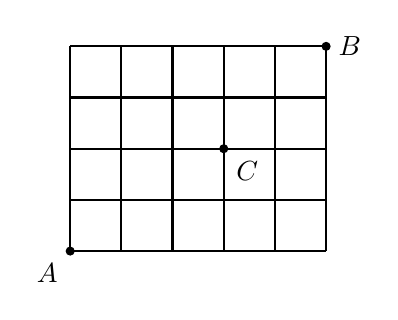
\begin{tikzpicture}[scale=0.65]
  \draw[line width=0.8pt] (0,0) grid (5,4);
  \filldraw (0,0) circle (2.2pt) node[below left=1pt] {$A$};
  \filldraw (5,4) circle (2.2pt) node[right=1pt] {$B$};
  \filldraw (3,2) circle (2.2pt) node[below right=1pt] {$C$};
\end{tikzpicture}
\par\vspace{0.3em}
{\small 圖 3-3}
\end{minipage}

\vspace{0.4em}
\noindent
$\dbinom{5}{3}\dbinom{4}{2}$ 條，故所求機率為 $\dbinom{5}{3}\dbinom{4}{2} \Bigg/ \dbinom{9}{5} = \dfrac{5!}{3!\,2!} \dfrac{4!}{2!\,2!} \dfrac{5!\,4!}{9!} = \dfrac{10}{21}$．\hfill\#

\vspace{1em}
\noindent\textbf{〔例 7〕}（重複試驗）擲硬幣 10 次，出現正、反面各 5 次的機率是多少？

\indent\textbf{解}\quad 擲硬幣 10 次可能出現的情形共有 $2^{10} = 1024$ 種，出現正、反面各 5 次的情形共有 $C_5^{10} = \dfrac{10!}{5!\,5!} = 252$，因此所求機率為 $\dfrac{252}{1024} = \dfrac{63}{256} \approx \dfrac{1}{4}$．\hfill\#

\vspace{0.8em}
\noindent\textbf{〔註〕}這個例子的答案接近 $1/4$，似乎有點令人驚異．因為每次出現正反面的機會各半，在重複試驗我們也就期待正反面出現的次數各半．這個例子說明正反面出現次數相等的機會並不大．實際上如果我們只期待正反面出現次數相近的話，則機會就會大為增加．出現正面 4 次反面 6 次的機率為 $C_4^{10}\left(\dfrac{1}{2}\right)^{10}$，而出現正面 6 次反面 4 次的機率為 $C_6^{10}\left(\dfrac{1}{2}\right)^{10}$．因此這三種情形（出現正面 4 至 6 次）的機率則為
\[
(C_4^{10} + C_5^{10} + C_6^{10})\left(\frac{1}{2}\right)^{10} = \frac{672}{1024} \approx 0.66.
\]

重複試驗時，如果各次試驗皆不受以前試驗的影響，則在整個試驗（重複 $n$ 次）中某一事件的機率顯然就等於在各次試驗中有關機率的乘積，舉例說明如下．

\vspace{1em}
\noindent\textbf{【論例 6】} 擲骰子 10 次，恰好出現 7 次 6 點的機率是多少？出現至少 7 次 6 點的機率又是多少？

\indent\textbf{解}\quad 這也是重複試驗的問題，我們可以依照剛才的說明求解．每次出現 6 點的機率為 $1/6$，出現其他點數的機率為 $5/6$，設想前 7 次皆出現 6 點，後 3 次皆為其他點數，則此一基本事件的機率為 $\left(\dfrac{1}{6}\right)^7 \left(\dfrac{5}{6}\right)^3$．

由排列可得 $C_7^{10}$ 種情形，因此恰好出現 7 次 6 點的機率為
\[
C_7^{10} \left(\frac{1}{6}\right)^7 \left(\frac{5}{6}\right)^3.
\]

\indent 同理求出恰好出現 8 次 6 點的機率為 $C_8^{10} \left(\dfrac{1}{6}\right)^8 \left(\dfrac{5}{6}\right)^2$

\indent 恰好出現 9 次 6 點的機率為 $C_9^{10} \left(\dfrac{1}{6}\right)^9 \left(\dfrac{5}{6}\right)$

\indent 恰好出現 10 次 6 點的機率為 $C_{10}^{10} \left(\dfrac{1}{6}\right)^{10}$

因此出現至少 7 次 6 點的機率為
\[
C_7^{10} \left(\frac{1}{6}\right)^7 \left(\frac{5}{6}\right)^3 + C_8^{10} \left(\frac{1}{6}\right)^8 \left(\frac{5}{6}\right)^2 + C_9^{10} \left(\frac{1}{6}\right)^9 \left(\frac{5}{6}\right) + C_{10}^{10} \left(\frac{1}{6}\right)^{10}.
\]

上例中前一個答案恰好就是下列二項展開式
\begin{align*}
\left(\frac{5}{6} + \frac{1}{6}\right)^{10} = & \ C_0^{10} \left(\frac{5}{6}\right)^{10} + C_1^{10} \left(\frac{5}{6}\right)^9 \left(\frac{1}{6}\right) + C_2^{10} \left(\frac{5}{6}\right)^8 \left(\frac{1}{6}\right)^2 \\
& + C_3^{10} \left(\frac{5}{6}\right)^7 \left(\frac{1}{6}\right)^3 + C_4^{10} \left(\frac{5}{6}\right)^6 \left(\frac{1}{6}\right)^4 \\
& + C_5^{10} \left(\frac{5}{6}\right)^5 \left(\frac{1}{6}\right)^5 + C_6^{10} \left(\frac{5}{6}\right)^4 \left(\frac{1}{6}\right)^6 + C_7^{10} \left(\frac{5}{6}\right)^3 \left(\frac{1}{6}\right)^7 \\
& + C_8^{10} \left(\frac{5}{6}\right)^2 \left(\frac{1}{6}\right)^8 + C_9^{10} \left(\frac{5}{6}\right) \left(\frac{1}{6}\right)^9 + C_{10}^{10} \left(\frac{1}{6}\right)^{10}
\end{align*}
中的第八項，而最後的答案就是第八至十一項的和，由這個例子可以看出，這一類型的重複試驗問題，我們也可以利用二項展開式來計算．

\vspace{1em}
\noindent\textbf{【論例 7】} (i) 袋中有三紅球，三白球，甲、乙二人輪流採取，每次取一球不放回，誰先取得紅球為獲勝．如果甲先開始，甲、乙二人獲勝的機率各為多少？

(ii) 如每次取出之球隨卽放回，則二人獲勝的機率又各為多少？

\indent\textbf{解}\quad (i) 我們考慮甲可能獲勝的情形：

第一次甲卽取得紅球，機率為 $\dfrac{3}{6} = \dfrac{1}{2}$．

第一次甲取白球，第二次乙取白球，第三次甲取紅球，機率為
\[
\frac{3}{6} \cdot \frac{2}{5} \cdot \frac{3}{4} = \frac{3}{20}.
\]
因此甲獲勝的機率為 $\dfrac{1}{2} + \dfrac{3}{20} = \dfrac{13}{20}$，乙獲勝的機率為 $1 - \dfrac{13}{20} = \dfrac{7}{20}$．

(ii) 第一次甲卽取得紅球之機率為 $\dfrac{1}{2}$，第一次甲取白球，第二次乙取白球，第三次甲取紅球之機率為 $\left(\dfrac{1}{2}\right)^3$，依此類推，可知甲獲勝之機率為
\[
\frac{1}{2} + \left(\frac{1}{2}\right)^3 + \left(\frac{1}{2}\right)^5 + \left(\frac{1}{2}\right)^7 + \cdots\cdots = \frac{1}{2}\left[1 + \frac{1}{4} + \left(\frac{1}{4}\right)^2 + \left(\frac{1}{4}\right)^3 + \cdots\cdots\right] = \frac{1}{2} \cdot \frac{1}{1 - \frac{1}{4}} = \frac{2}{3}.
\]
因為甲乙二人永遠都取白球的機率為 $\left(\dfrac{1}{2}\right)^n \longrightarrow 0$，當 $n \longrightarrow \infty$ 時，所以乙獲勝之機率為 $1 - \dfrac{2}{3} = \dfrac{1}{3}$．\hfill\#

\vspace{1em}
\noindent\textbf{**【例 8】}（不同條件下分配問題的機率）

設 $0 \le r \le n$，在下列四種不同的條件下，將 $r$ 個球隨意放入 $n$ 個編號不同的箱子中：
\begin{enumerate}[(1), itemsep=0.1em, topsep=0.2em]
  \item $r$ 個不同的球，每箱放入個數不限．
  \item $r$ 個不同的球，每箱至多放一個．
  \item $r$ 個相同的球，每箱至多放一個．
  \item $r$ 個相同的球，每箱放入個數不限．
\end{enumerate}
試求在指定的 $r$ 個箱子中，每箱恰有一球的機率．

\medskip
\indent\textbf{解}\quad 設樣本空間為 $S$，給定事件為 $A$．對於上列四種情況，我們利用上一章的排列與組合方法求出 $|S|$ 及 $|A|$，從而得到所求的機率 $P(A)$：

\begin{center}
\renewcommand{\arraystretch}{1.5}
\begin{tabular}{ccccc}
 & $|S|$ & $|A|$ & $P(A)$ & \\
\hline
(1) & $n^r$ & $r!$ & $r!/n^r$ & (Maxwell-Boltzmann統計) \\
(2) & $P_r^n$ & $r!$ & $r!/P_r^n$ & \multirow{2}{*}{$\left.\rule{0pt}{1.6em}\right\} = 1/C_r^n\text{ (Dirac-Fermi 統計)}$} \\
(3) & $C_r^n$ & $1$ & $1/C_r^n$ & \\
(4) & $C_r^{n+r-1}$ & $1$ & $1/C_r^{n+r-1}$ & (Bose-Einstein 統計) \\
\hline
\end{tabular}
\end{center}

\vspace{0.5em}
\noindent\textbf{〔註〕}這種分配問題在統計物理上非常重要．統計物理中討論各種物理粒子關於某些性質的分佈情形．Maxwell-Boltzmann 的古典統計物理將所觀察的粒子視為可以區分的，他們的統計方法適用於氣體分子等的討論．Dirac-Fermi 假設所觀察的粒子不可區分，且沒有兩個粒子分佈在同一狀態；這種方法適用於電子、中子、質子的研究．Bose-Einstein 的方法中亦將所觀察的粒子視為不可區分；這種統計方法適用的範圍包含原子核、光子等．

\vspace{0.8em}
我們現在利用等差數列的方法來求出前面所提到的全盤獲勝問題的答案．

\vspace{1em}
\noindent\textbf{【論例 8】} 設甲有 $m$ 元，乙有 $n$ 元，二人作一枚公正的硬幣遊戲，出現正面則甲贏乙一元，出現反面則乙贏甲一元，問甲將乙所有的全部資本 $n$ 元贏去的機率為多少？

\indent\textbf{解}\quad 令 $k = m + n$，則 $k$ 是一個定數，設甲有 $i$ 元（$0 \le i \le k$），乙有 $(k - i)$ 元時，甲將乙的全部款項 $(k - i)$ 元贏去的機率為 $P_i$．顯然
\[
P_0 = 0 \text{ 及 } P_k = 1.
\]
由於二人獲勝的機會均等，故有
\[
P_i = \frac{1}{2} P_{i+1} + \frac{1}{2} P_{i-1}, \quad 1 \le i \le k - 1.
\]
上式可改寫為
\[
P_i - P_{i-1} = P_{i+1} - P_i, \quad 1 \le i \le k - 1.
\]
由上式可知 $P_i$, $i = 0, 1, \dots, k$ 是一個等差數列，首項 $P_0 = 0$，末項 $P_k = 1$．因此一般項~$P_i = \dfrac{i}{k}$．$i = m$ 時 $P_m = \dfrac{m}{m+n}$ 卽為所求的機率．\hfill\#

\vspace{1.5em}
% ==============================================================================
% 習題 III-2
% ==============================================================================
\subsubsection*{習題 III-2}\label{sec:b5-ex3-2}

\begin{enumerate}[label=\textbf{\arabic*.}]
  \item 打橋牌時，用的牌是黑桃、紅心、方塊、梅花各 13 張，每人分 13 張，問所分的 13 張中有 12 張是黑桃的機率是多少？13 張都不是黑桃的機率是多少？至少有一張是紅心的機率是多少？
  \item 已知在一箱中有 60 個燈泡，其中有 8 個燈絲斷了，現作逐個檢查，問檢查到第三個時，是第二個斷了燈絲的燈泡的機率是多少？
  \item 將 $1, 2, \dots, 10$ 分別寫在同樣的 10 張紙牌上，放入一個暗袋內任意取出兩張紙牌，試計算下述各事件的機率．
  \begin{enumerate}[label=(\arabic*)]
    \item 它們的數目差為 1．
    \item 兩張牌的數目都不超過 5．
    \item 兩張均為偶數牌．
    \item 至少有一張牌寫的是 1 或 5．
    \item 兩張數目的差不超過 2．
  \end{enumerate}
  \item 某班上有 40 人身高均不相等，從點名簿任意叫出 5 個人．
  \begin{enumerate}[label=(\arabic*)]
    \item 班上最高的和最低的同學被叫出的機率是多少？
    \item 被叫出的 5 人中第三位同學是全班第五高的機率多少？
    \item 班上最高的 4 人中有 3 人被叫出的機率是多少？
  \end{enumerate}
  \item 將四張寫好收信人名的信隨意地放入四張寫好收信人名及地址的信封內，求下述各事件的機率：
  \begin{enumerate}[label=(\arabic*)]
    \item 至少有一張信放對了信封．
    \item 沒有一張信放對了信封．
    \item 將信與信封的個數改為 $n$ 時，(1)，(2)的答案如何？
  \end{enumerate}
  \item 設某型飛機用引擎連續飛行 8 小時不發生故障的機率為 0.99，如果雙引擎飛機只要有一引擎正常就可以飛行，四引擎飛機，只要其中兩個引擎正常就可以飛行，現假設一引擎是否發生故障與其它引擎無關：
  \begin{enumerate}[label=(\arabic*)]
    \item 試證兩種飛機同時飛行 8 小時的期間內，雙引擎飛機因引擎失事的機率為四引擎飛機失事機率的 25 倍．
    \item 計算上述兩種飛機因引擎失常而失事的機率．\phantomsection\label{note:b5-ch3-p110-q6-subnum}\footnote{【原書註記/校訂】：原書第 110 頁習題 III-2 第 6 題子題序號印為「(1) ... (3) ... (3)」，其第三子題敘述「(2)中若引擎故障...」明指前一題為第 (2) 子題，顯係排印編號訛誤，茲逕予更正為 (2)．}
    \item (2)中若引擎故障的機率是 $p$ 時，答案如何？
  \end{enumerate}
\end{enumerate}

% ==============================================================================
% *§ III-3 幾何機率
% ==============================================================================
\subsection{*幾何機率}\label{sec:b5-3-3}

在以上所討論中，我們假設一項試驗中所有可能發生的現象為有限多個，而且各個現象發生的機會都相等，這樣我們可以很合理地定義事件的機率．這種直觀的想法也可以加以引伸，應用到有關幾何圖形的討論．但是此時用來定義機率的不是樣本點的個數，而是幾何圖形的長度，面積或體積等度量\footnote{* 社會組可略去不授，供讀者參考．}．

\medskip
\noindent\textbf{〔例 9〕} 設圓形鏢靶的半徑為 $30$ 公分，紅心的半徑為 $5$ 公分．若未經瞄準偶然擲中鏢靶，問此鏢中紅心的機率是多少？

\noindent\textbf{解}\quad 所求機率為二圓形面積之比，卽
\[
\frac{\pi \cdot 5^2}{\pi \cdot 30^2} = \frac{1}{36}. \tag*{\#}
\]

\medskip
\noindent\textbf{〔例 10〕} 袋中有 $10$ 個球，分別標記 $0, 1, 2, 3, 4, 5, 6, 7, 8, 9$ 各數字，每次採取一球，記下數字後立即放回，假設我們一次，二次，……無限多次地做下去（實際上，永遠不能做到），則得到一串數字．如果在最前面加一個小數點，就得到一個在 $0$ 與 $1$ 之間的實數；試問得到 $0.500\dots\dots$ 的機率是多少？得到一個在 $0.25$ 與 $0.5$ 之間的實數的機率又是多少？

\noindent\textbf{解}\quad $0$ 與 $1$ 之間每一實數都是一個樣本點，所以樣本空間中有無限多個樣本點．因此要得到其中某一個實數的機率為 $0$，要得到 $0.500\dots\dots$ 的機率當然也是 $0$．要得到 $0.25$ 與 $0.5$ 之間實數的機率則可考慮長度的比，卽為
\[
\frac{0.5 - 0.25}{1 - 0} = 0.25.
\]

\medskip
\noindent\textbf{〔例 11〕} 轉盤遊戲用一指針在圓盤上轉動．設圓盤半徑為 $a$，頭獎部分的圓弧長為 $b$，試求中頭獎的機率．

\noindent\textbf{解}\quad 所求機率為弧長的比，卽 $\dfrac{b}{2\pi a}$\phantomsection\label{note:b5-ch3-p111-2pia}\footnote{【原書註記/校訂】：原書此處分母字模受損作「$2\text{--}a$」，依圓周長公式 $2\pi a$ 校訂為 $2\pi a$．}．如利用面積的比，亦得同樣結果．

\medskip
\noindent\textbf{〔例 12〕（約會問題）} 某君與女友相約在下午五時至六時之間在公園門口見面，先到的人應等候 $20$ 分鐘，求二人在公園門口相遇的機率．

\noindent\textbf{解}\quad 我們以下午 5 時作為時間起點．設某君到達公園門口的時間為 $x$，女友到達的時間為 $y$，則以分鐘為單位時
\[
0 \le x \le 60,\quad 0 \le y \le 60.
\]
二人到達的時間構成一個樣本點 $(x, y)$，在平面直角坐標系上為一邊長 60 的正方形，亦卽本問題的樣本空間．又由題意可知二人相遇的條件為
\[
|x - y| \le 20.
\]

\begin{figure}[H]
\centering
\begin{tikzpicture}[scale=0.07]
  % Axes
  \draw[-Stealth, thick] (-5, 0) -- (78, 0) node[right=2pt] {$x$};
  \draw[-Stealth, thick] (0, -5) -- (0, 78) node[above=2pt] {$y$};
  \node[below left=2pt] at (0, 0) {$O$};
  
  % Tick marks and values
  \draw[thick] (20, 1.5) -- (20, -1.5) node[below=3pt] {$20$};
  \draw[thick] (60, 1.5) -- (60, -1.5) node[below=3pt] {$60$};
  \draw[thick] (1.5, 20) -- (-1.5, 20) node[left=3pt] {$20$};
  \draw[thick] (1.5, 60) -- (-1.5, 60) node[left=3pt] {$60$};
  
  % Shaded region |x - y| <= 20
  \fill[pattern=horizontal lines, pattern color=black!70] 
    (0, 0) -- (20, 0) -- (60, 40) -- (60, 60) -- (40, 60) -- (0, 20) -- cycle;
  
  % Boundary lines of region
  \draw[thick] (0, 20) -- (40, 60);
  \draw[thick] (20, 0) -- (60, 40);
  
  % Square frame
  \draw[thick] (0, 0) rectangle (60, 60);
  
  % Point labels
  \node[above=3pt] at (40, 60) {$(40, 60)$};
  \node[right=3pt] at (60, 40) {$(60, 40)$};
\end{tikzpicture}
\end{figure}

在正方形中且滿足此不等式的區域如圖中陰影部分所示．因此所求機率卽為正方形面積與陰影部分面積之比，等於
\[
\frac{60^2 - 40^2}{60^2} = \frac{5}{9}.
\]

\medskip
\noindent\textbf{**〔例 13〕（擲針問題）} 在平面上作無限多根平行直線，間隔皆為 $2a$，將一長度為 $2b$ ($b \le a$) 的針擲到平面上，此針可與平行直線相交或不相交．求此針與所劃直線相交的機率．

\noindent\textbf{解}\quad 設針的中心到最近直線的距離為 $x$，夾角為 $\varphi$\phantomsection\label{note:b5-ch3-p113-phi}\footnote{【原書註記/校訂】：原書此處與下文使用希臘字母 $\varphi$（亦作 $\phi$），但在次行誤植為 $\psi$（「$0 \le \psi < \pi$」），茲統一校訂為 $\varphi$．}，則 $0 \le x \le a$，$0 \le \varphi < \pi$．針的位置完全由 $x$ 及 $\varphi$ 所決定，所以 $(x, \varphi)$ 表示一個樣本點，

\begin{figure}[H]
\centering
\begin{tikzpicture}[scale=1.4]
  % Parallel horizontal lines
  \draw[thick] (-0.8, 1.8) -- (4.8, 1.8);
  \draw[thick] (-0.8, 0) -- (4.8, 0);
  
  % Distance 2a
  \draw[thick, Stealth-Stealth] (0.2, 0) -- (0.2, 1.8);
  \node[fill=white, inner sep=2pt] at (0.2, 0.9) {$2a$};
  
  % Needle
  % Center C at (2.4, 1.1)
  \coordinate (C) at (2.4, 1.1);
  % Upper line y = 1.8. Distance x = 0.7.
  % Angle = 38 deg.
  % Intersection with y = 1.8: x_int = 2.4 + 0.7 / tan(38) = 2.4 + 0.896 = 3.296
  \coordinate (P) at (3.296, 1.8);
  \coordinate (N_bot) at ($(C) - ({1.3*cos(38)}, {1.3*sin(38)})$);
  \coordinate (N_top) at ($(C) + ({1.5*cos(38)}, {1.5*sin(38)})$);
  
  \draw[very thick] (N_bot) -- (N_top);
  
  % Vertical distance x
  \draw[thick] (C) -- (2.4, 1.8);
  \node[left=2pt] at (2.4, 1.45) {$x$};
  \filldraw (C) circle (1.5pt);
  
  % Angle phi arc inside the triangle (below horizontal line, between needle and line)
  \draw[thick] (P) ++(180:0.45) arc (180:218:0.45);
  \node at ($(P) + (199:0.7)$) {$\varphi$};
\end{tikzpicture}
\caption*{圖 3-5-1}\phantomsection\label{note:b5-ch3-p113-fig-num}\footnote{【原書註記/校訂】：原書圖號作「圖 3-5-1」與「圖 3-5-2」，疑承襲原教材早期章節編號（如第 5 節），本節標題為 §III-3，茲存其舊並予註記．}
\label{fig:b5-3-5-1}
\end{figure}

\noindent 點，而樣本空間卽為上述長方形，如下圖所示，若針與直線相交，則
\[
x \le b \sin\varphi.
\]

\begin{figure}[H]
\centering
\begin{tikzpicture}[scale=1.3]
  % Axes
  \draw[-Stealth, thick] (-0.4, 0) -- (4.2, 0) node[right=2pt] {$\varphi$};
  \draw[-Stealth, thick] (0, -0.3) -- (0, 2.5) node[above=2pt] {$x$};
  \node[below left=2pt] at (0, 0) {$O$};
  
  % Rectangle width pi (approx 3.1416), height a (approx 2.0)
  \def\piVal{3.14159}
  \def\aHeight{2.0}
  \def\bAmp{1.3}
  
  % Shaded sine area
  \fill[pattern=horizontal lines, pattern color=black!70]
    plot[domain=0:\piVal, samples=60] (\x, {\bAmp*sin(\x r)}) -- (0, 0) -- cycle;
  
  % Curve x = b sin \varphi
  \draw[very thick] plot[domain=0:\piVal, samples=60] (\x, {\bAmp*sin(\x r)});
  
  % Rectangle frame
  \draw[thick] (0, 0) rectangle (\piVal, \aHeight);
  
  % Labels
  \node[left=3pt] at (0, \aHeight) {$a$};
  \node[below=3pt] at (\piVal, 0) {$\pi$};
  \node[above=4pt] at ({\piVal/2}, \bAmp) {$x = b \sin\varphi$};
\end{tikzpicture}
\caption*{圖 3-5-2}
\label{fig:b5-3-5-2}
\end{figure}

長方形中滿足此不等式的部分卽在正弦曲線 $x = b \sin\varphi$ 下方的陰影區域．因此所求機率為二者面積之比，等於 $\dfrac{2b}{\pi a}$．（陰影部分的面積等於 $2b$，係利用積分求出）．

這個問題係由 J. Buffon（十八世紀法國科學家）所作，後來應用於砲彈落點的研究．

% ==============================================================================
% 習題 III-3
% ==============================================================================
\subsubsection*{習題 III-3}\label{sec:b5-ex3-3}

\begin{enumerate}[label=\textbf{\arabic*.}]
  \item 某君與女友相約在下午四時到六時在公園門口見面：
  \begin{enumerate}[label=(\arabic*)]
    \item 約定任何人先到都等候 $30$ 分鐘，問兩人相遇的機率是多少？
    \item 若約定某君先到時等 $30$ 分鐘，女友先到時不等，則兩人相遇的機率是多少？
    \item 若約定某君先到時應等 $30$ 分鐘，女友先到時只等 $20$ 分鐘，問兩人相遇的機率是多少？
  \end{enumerate}

  \item 設一圓形鈕扣的直徑是 $2$ 公分，一圍棋盤的直線與橫線的間隔都是 $3$ 公分，將鈕扣任意擲入棋盤內．
  \begin{enumerate}[label=(\arabic*)]
    \item 鈕扣不接觸到棋盤線的機率是多少？
    \item 鈕扣接觸到棋盤線的機率是多少？
  \end{enumerate}

  \item 假設一城市的電線架設成棋盤形，就是說縱的和橫的，每隔 $100$ 公尺都有直線形電線，若以一有效半徑為 $30$ 公尺的炸彈投入該城市，則炸中電線的機率是多少？

  \item 方程式 $x^2 + px + q = 0$ 的係數 $p, q$ 是分別由骰子 $A$ 與骰子 $B$ 所擲出的點數代入．問該方程的根為虛根的機率是多少？

  \item 上題中，$A, B$ 是由標明 $0, 1, 2, \ldots, 9$ 十個數的十面體（各面都是全等的三角形，像一顆鑽石）所擲出時，答案如何？
\end{enumerate}
